% package inclusion and set up of the document
\documentclass[12pt,twoside,a4paper,titlepage]{report}
\usepackage{etex}
% Select encoding of your inputs.
\usepackage[utf8]{inputenc}

% Make latex understand and use the typographic
% rules of the language used in the document.
\usepackage[english]{babel}

% Use the vector font Latin Modern which is going
% to be the default font in latex in the future.
\usepackage{lmodern}

% Choose the font encoding
\usepackage[T1]{fontenc}

% load a colour package
\usepackage{xcolor}
\definecolor{aaublue}{RGB}{33,26,82}  % dark blue
\definecolor{white}{RGB}{255,255,255} % define color white
\definecolor{black}{RGB}{0,0,0}       % define color black
\definecolor{coolblue}{RGB}{32,95,128}
\definecolor{mygreen}{RGB}{0,0.6,0}
\definecolor{mygray}{RGB}{0.5,0.5,0.5}
\definecolor{mymauve}{RGB}{0.58,0,0.82}
\definecolor{lbcolor}{RGB}{0.9,0.9,0.9}
\definecolor{listinggray}{gray}{0.9}


% The standard graphics inclusion package
\usepackage[cc]{titlepic}
\usepackage{graphicx}
\graphicspath{{./figures/}}
\usepackage{adjustbox}

% Set up how figure and table captions are displayed
\usepackage{caption}
\captionsetup{%
  font=footnotesize,% set font size to footnotesize
  labelfont=bf % bold label (e.g., Figure 3.2) font
}

% Enable row combination in tables
\usepackage{multirow}

% Make space between table lines and text
\renewcommand{\arraystretch}{1.5}

% Make the standard latex tables look so much better
\usepackage{array,booktabs}

% Enable the use of frames around, e.g., theorems
% The framed package is used in the example environment
\usepackage{framed}
\usepackage{colortbl}
\usepackage{longtable}
\usepackage{xcolor}

\usepackage{textcomp}

%%%%%%%%%%%%%%%%%%%%%%%%%%%%%%%%%%%%%%%%%%%%%%%%
% Mathematics
%%%%%%%%%%%%%%%%%%%%%%%%%%%%%%%%%%%%%%%%%%%%%%%%
% Defines new environments such as equation,
% align and split 
\usepackage{amsmath}
\usepackage{relsize}
% Adds new math symbols
\usepackage{amssymb}
% Use theorems in your document
% The ntheorem package is also used for the example environment
% When using thmmarks, amsmath must be an option as well. Otherwise \eqref doesn't work anymore.
\usepackage[framed,amsmath,thmmarks]{ntheorem}

%%%%%%%%%%%%%%%%%%%%%%%%%%%%%%%%%%%%%%%%%%%%%%%%
% Page Layout
%%%%%%%%%%%%%%%%%%%%%%%%%%%%%%%%%%%%%%%%%%%%%%%%
% Change margins, papersize, etc of the document
% \usepackage[
%   left=25mm,% left margin on an odd page %tidligere 25mm for baade right og left
%   right=25mm,% right margin on an odd page
%   top=35mm,
%   ]{geometry}
  
% Modify how \chapter, \section, etc. look
% The titlesec package is very configureable

\usepackage{titlesec, blindtext, color}
%\color{gray75}{gray}{0.75}
\newcommand{\hsp}{\hspace{20pt}}
\titleformat{\chapter}[hang]{\huge\bfseries}{\thechapter\hsp\textcolor{aaublue}{|}\hsp}{0pt}{\huge\bfseries}


% \usepackage{titlesec}
% \makeatletter
% \def\ttl@mkchap@i#1#2#3#4#5#6#7{%
%     \ttl@assign\@tempskipa#3\relax\beforetitleunit
%     \vspace{\@tempskipa}%<<<<<< REMOVE THE * AFTER \vspace
%     \global\@afterindenttrue
%     \ifcase#5 \global\@afterindentfalse\fi
%     \ttl@assign\@tempskipb#4\relax\aftertitleunit
%     \ttl@topmode{\@tempskipb}{%
%         \ttl@select{#6}{#1}{#2}{#7}}%
%     \ttl@finmarks  % Outside the box!
%     \@ifundefined{ttlp@#6}{}{\ttlp@write{#6}}}
% \makeatother

\titlespacing{\chapter}{-15pt}{0pt}{10pt}
\titlespacing{\section}{0pt}{0pt}{5pt}
\titlespacing{\subsection}{0pt}{8pt}{5pt}
\titlespacing{\subsubsection}{0pt}{6pt}{0pt}

% \titleformat*{\section}{\normalfont\Large\bfseries\color{aaublue}}
% \titleformat*{\subsection}{\normalfont\large\bfseries\color{aaublue}}
% \titleformat*{\subsubsection}{\normalfont\normalsize\bfseries\color{aaublue}}
% \titleformat*{\paragraph}{\normalfont\normalsize\bfseries\color{aaublue}}
% \titleformat*{\subparagraph}{\normalfont\normalsize\bfseries\color{aaublue}}

%Formatting chapter headers. Predefined styles that can be used as option to the package: Sonny, Lenny, Glenn, Conny, Rejne, Bjarne, PetersLenny and Bjornstrup
% \usepackage[Sonny]{fncychap}

% Change the headers and footers
\usepackage{fancyhdr}
\setlength{\headheight}{15pt}
\pagestyle{fancy}
\fancyhf{} %delete everything
\renewcommand{\headrulewidth}{0pt} %remove the horizontal line in the header
\fancyhead[RO,LE]{\color{aaublue}\small\nouppercase\leftmark} %even page - chapter title

\fancyhead[LO]{}
\fancyhead[RE]{} 
\fancyhead[CE]{}
\fancyhead[CO]{}

% change first page of all chapters header and footer to fancy style
\makeatletter
\let\ps@plain\ps@fancy
\makeatother

% Do not stretch the content of a page. Instead,
% insert white space at the bottom of the page
\raggedbottom

% Enable arithmetics with length. Useful when typesetting the layout.
\usepackage{calc}

%%%%%%%%%%%%%%%%%%%%%%%%%%%%%%%%%%%%%%%%%%%%%%%%
% Bibliography
%%%%%%%%%%%%%%%%%%%%%%%%%%%%%%%%%%%%%%%%%%%%%%%%
%setting references (using numbers) and supporting i.a. Chicargo-style:
\usepackage{etex}
\usepackage{etoolbox}
\usepackage{keyval}
\usepackage{ifthen}
\usepackage{url}
\usepackage{csquotes}
\usepackage[backend=biber, url=true, doi=true, style=numeric, sorting=none]{biblatex}
\bibliography{bibliography.bib}

%%%%%%%%%%%%%%%%%%%%%%%%%%%%%%%%%%%%%%%%%%%%%%%%
% Misc
%%%%%%%%%%%%%%%%%%%%%%%%%%%%%%%%%%%%%%%%%%%%%%%%

% Add bibliography and index to the table of
% contents
% %\usepackage[nottoc, notlof, notlot]{tocbibind}
\usepackage{tocloft}

% Add the command \pageref{LastPage} which refers to the
% page number of the last page
\setlength{\cftbeforetoctitleskip}{0 cm}

% Enables figures with text wrapped tightly around it 
\usepackage{wrapfig}

%%% Section debth included in table of contents (1 = down to sections) %%%
\setcounter{tocdepth}{2}

%%% Section debth for numbers (1 = down to sections) %%%
\setcounter{secnumdepth}{2}

%%%%%%%%%%%%%%%%%%%%%%%%%%%%%%%%%%%%%%%%%%%%%%%%
% Hyperlinks
%%%%%%%%%%%%%%%%%%%%%%%%%%%%%%%%%%%%%%%%%%%%%%%%

% Enable hyperlinks and insert info into the pdf
% file. Hypperref should be loaded as one of the 
% last packages
\usepackage{nameref}
\usepackage{hyperref}
\hypersetup{%
  %pdfpagelabels=true,%
  plainpages=false,%
  pdfauthor={Author(s)},%
  pdftitle={Title},%
  pdfsubject={Subject},%
  bookmarksnumbered=true,%
  colorlinks,%
  citecolor=aaublue,%
  filecolor=aaublue,%
  linkcolor=aaublue,% you should probably change this to black before printing
  urlcolor=aaublue,%
  pdfstartview=FitH%
}

%enables code-examples
\usepackage{listings}
\lstset{
  backgroundcolor=\color{white},   % choose the background color; you must add \usepackage{color} or \usepackage{xcolor}
  basicstyle=\footnotesize,        % the size of the fonts that are used for the code
  breakatwhitespace=false,         % sets if automatic breaks should only happen at whitespace
  breaklines=true,                 % sets automatic line breaking
  captionpos=t,                    % sets the caption-position to bottom
  commentstyle=\color{mygreen},    % comment style
  deletekeywords={...},            % if you want to delete keywords from the given language
  escapeinside={\%*}{*)},          % if you want to add LaTeX within your code
  extendedchars=true,              % lets you use non-ASCII characters; for 8-bits encodings only, does not work with UTF-8
  frame=single,                    % adds a frame around the code
  keepspaces=true,                 % keeps spaces in text, useful for keeping indentation of code (possibly needs columns=flexible)
  keywordstyle=\color{blue},       % keyword style
  language=C++,                 % the language of the code
  morekeywords={*,...},            % if you want to add more keywords to the set
  numbers=left,                    % where to put the line-numbers; possible values are (none, left, right)
  numbersep=5pt,                   % how far the line-numbers are from the code
  numberstyle=\tiny\color{mygray}, % the style that is used for the line-numbers
  rulecolor=\color{black},         % if not set, the frame-color may be changed on line-breaks within not-black text (e.g. comments (green here))
  showspaces=false,                % show spaces everywhere adding particular underscores; it overrides 'showstringspaces'
  showstringspaces=false,          % underline spaces within strings only
  showtabs=false,                  % show tabs within strings adding particular underscores
  stepnumber=1,                    % the step between two line-numbers. If it's 1, each line will be numbered
  stringstyle=\color{mymauve},     % string literal style
  tabsize=2,                       % sets default tabsize to 2 spaces
  title=\lstname                   % show the filename of files included with \lstinputlisting; also try caption instead of title
backgroundcolor=\color{lbcolor},
  tabsize=4,
  rulecolor=,
  language=C,
        basicstyle=\scriptsize,
        upquote=true,
        aboveskip={1.5\baselineskip},
        columns=fixed,
        showstringspaces=false,
        extendedchars=true,
        breaklines=true,
        prebreak = \raisebox{0ex}[0ex][0ex]{\ensuremath{\hookleftarrow}},
        frame=single,
        showtabs=false,
        numbers=left,
        captionpos=b,
        numbersep=5pt,
        numberstyle=\tiny\color{mygray},
        showspaces=false,
        showstringspaces=false,
        identifierstyle=\ttfamily,
        keywordstyle=\color[rgb]{0,0,1},
        commentstyle=\color[rgb]{0.133,0.545,0.133},
        stringstyle=\color[rgb]{0.627,0.126,0.941},
}

\usepackage{textcomp}
\usepackage{float}
\usepackage{caption}
\usepackage{subcaption}
\usepackage{siunitx}
\sisetup{decimalsymbol=comma}
\sisetup{detect-weight}

\usepackage{enumitem}
\usepackage{pdfpages}
\usepackage{lastpage}
\usepackage{epstopdf}

% Figures - TIKZ
\usepackage{tikz}
\usepackage[americanresistors,americaninductors,americancurrents, americanvoltages]{circuitikz}
% special personal macros
%Creates the aau titlepage
\newcommand{\aautitlepage}[3]{%
  {
    %set up various length
    \ifx\titlepageleftcolumnwidth\undefined
      \newlength{\titlepageleftcolumnwidth}
      \newlength{\titlepagerightcolumnwidth}
    \fi
    \setlength{\titlepageleftcolumnwidth}{0.5\textwidth-\tabcolsep}
    \setlength{\titlepagerightcolumnwidth}{\textwidth-2\tabcolsep-\titlepageleftcolumnwidth}
    %create title page
    \thispagestyle{empty}
    \noindent%
    \begin{tabular}{@{}ll@{}}
      \parbox{\titlepageleftcolumnwidth}{
        \iflanguage{danish}{%
          
\includegraphics[width=\titlepageleftcolumnwidth]{aau_logo_da.pdf}
        }{%
          
\includegraphics[width=\titlepageleftcolumnwidth]{aau_logo_en.pdf}
        }
      } &
      \parbox{\titlepagerightcolumnwidth}{\raggedleft\sf\small
        #2
      }\bigskip\\
       #1 &
      \parbox[t]{\titlepagerightcolumnwidth}{%
      \textbf{Abstract:}\smallskip\par
        \fbox{\parbox{\titlepagerightcolumnwidth-2\fboxsep-2\fboxrule}{%
          #3
        }}
      }\\
    \end{tabular}
    \vfill
    \vspace{-0.5cm}
    \iflanguage{danish}{%
      \noindent{\footnotesize\emph{Rapportens indhold er frit tilgængeligt, men offentliggørelse (med kildeangivelse) må kun ske efter aftale med forfatterne.}}
    }{%
      \noindent{\footnotesize\emph{The content of this report is freely available, but publication (with reference) may only be pursued due to agreement with the author.}}
    }
    \clearpage
  }
}

%Create english project info
\newcommand{\englishprojectinfo}[8]{%
  \parbox[t]{\titlepageleftcolumnwidth}{
    \textbf{Title:}\\ #1\bigskip\par
    \textbf{Theme:}\\ #2\bigskip\par
    \textbf{Project Period:}\\ #3\bigskip\par
    \textbf{Project Group:}\\ #4\bigskip\par
    \textbf{Participant(s):}\\ #5\bigskip\par
    \textbf{Supervisor(s):}\\ #6\bigskip\par
    \textbf{Copies:} #7\bigskip\par
    \textbf{Page Numbers:} Fucking mange!\bigskip\par
    \textbf{Date of Completion:}\\ #8
  }
}

%Create danish project info
\newcommand{\danishprojectinfo}[8]{%
  \parbox[t]{\titlepageleftcolumnwidth}{
    \textbf{Title:}\\ #1\bigskip\par
    \textbf{Theme:}\\ #2\bigskip\par
    \textbf{Project Period:}\\ #3\bigskip\par
    \textbf{Project Group:}\\ #4\bigskip\par
    \textbf{Participants:}\\ #5\bigskip\par
    \textbf{Supervisor:}\\ #6\bigskip\par
    \textbf{Copies:} #7\bigskip\par
    \textbf{Page Numbers:} ??
    \bigskip\par
    \textbf{Date of Completion:}\\ #8
  }
}


\newcommand{\iic}[0]{I²C }

%%%%%%%%%%%%%%%%%%%%%%%%%%%%%%%%%%%%%%%%%%%%%%%%
%            An example environment            %
%%%%%%%%%%%%%%%%%%%%%%%%%%%%%%%%%%%%%%%%%%%%%%%%
\theoremheaderfont{\normalfont\bfseries}
\theorembodyfont{\normalfont}
\theoremstyle{break}
\def\theoremframecommand{{\color{aaublue!50}\vrule width 5pt \hspace{5pt}}}
\newshadedtheorem{exa}{Example}[chapter]
\newenvironment{example}[1]{%
		\begin{exa}[#1]
}{%
		\end{exa}
}

\makeatletter
\newcommand{\ChapterOutsidePart}{%
   \def\toclevel@chapter{-1}\def\toclevel@section{0}\def\toclevel@subsection{1}}
\newcommand{\ChapterInsidePart}{%
   \def\toclevel@chapter{0}\def\toclevel@section{1}\def\toclevel@subsection{2}}
\makeatother

\usepackage{bookmark}

\usepackage{mathtools}
\DeclarePairedDelimiter{\ceil}{\lceil}{\rceil}


%%%%%%%%%%%%%%%%%%%%%%%%%%%%%%%%%%%%%%%%%%%%%%%%%%%%%
%                  USEFULL MACROES                  %
%%%%%%%%%%%%%%%%%%%%%%%%%%%%%%%%%%%%%%%%%%%%%%%%%%%%%
%Units:
\newcommand{\unit}[1]{&& \left[\si{#1}\right]} %\newcommand{\unit}[1]{[\si{#1}]}             <<| Use these if you want equations to be
\newcommand{\unitWh}[1]{[\si{#1}]}             %\newcommand{\eq}[2]{&&\si{#1} &= \si{#2}&&}  <<| centered.. .. will be appear scrambled
\newcommand{\numUnit}[1]{\ \si{#1}&}           %                                               | from one equation to the next though..
%Equation:                                     %                                               | and does not work with long equations.. :/
\newcommand{\eq}[2]{\si{#1} &= \si{#2}}
\newcommand{\arw}{&& &\Updownarrow&&}
%Text:
\newcommand{\tx}[1]{\text{#1}}


%%%%%%%%%%%%%%%%%%%%%%%%%%%%%%%%%%%%%%%%%%%%%%%%%%%%%
%                  REFERENCES                       %
%%%%%%%%%%%%%%%%%%%%%%%%%%%%%%%%%%%%%%%%%%%%%%%%%%%%%

%Chapter
\newcommand{\chapref}[1]{\emph{Chapter \ref{#1}}} %:\textbf{ \nameref{#1}}}}
%Section
\newcommand{\secref}[1]{\emph{Section \ref{#1}}} %:\textbf{ \nameref{#1}}}}
%subSection
\newcommand{\subsecref}[1]{\emph{Subsection \ref{#1}}} %:\textbf{ \nameref{#1}}}}
%Appendix
\newcommand{\appref}[1]{\emph{Appendix \ref{#1}}} %:\textbf{ \nameref{#1}}}}
%Listings
\newcommand{\coderef}[1]{\emph{Listings: \ref{#1}}}
%Figure:
\newcommand{\figref}[1]{\emph{Figure \ref{#1}}}
%Table:
\newcommand{\tableref}[1]{\emph{Table \ref{#1}}}

%Equations:
%1 equation:
\renewcommand{\eqref}[1]{\emph{Equation (\ref{#1})}}
%2 equations:
\newcommand{\eqrefTwo}[2]{\emph{Equation (\ref{#1})} and \emph{(\ref{#2})}}
%3 equations:
\newcommand{\eqrefThree}[3]{\emph{Equation (\ref{#1})}, \emph{(\ref{#2})} and \emph{(\ref{#3})}}
%4 equations:
\newcommand{\eqrefFour}[4]{\emph{Equation (\ref{#1})}, \emph{(\ref{#2})}, \emph{(\ref{#3})} and \emph{(\ref{#4})}}
%5 equations:
\newcommand{\eqrefFive}[5]{\emph{Equation (\ref{#1})}, \emph{(\ref{#2})}, \emph{(\ref{#3})}, \emph{(\ref{#4})} and \emph{(\ref{#5})}}
%6 equations:
\newcommand{\eqrefSix}[6]{\emph{Equation (\ref{#1})}, \emph{(\ref{#2})}, \emph{(\ref{#3})}, \emph{(\ref{#4})}, \emph{(\ref{#5})} and \emph{(\ref{#6})}}
%7 equations:
\newcommand{\eqrefSeven}[7]{\emph{Equation (\ref{#1})}, \emph{(\ref{#2})}, \emph{(\ref{#3})}, \emph{(\ref{#4})}, \emph{(\ref{#5})}, \emph{(\ref{#6})} and \emph{(\ref{#7})}}

\begin{document}

\title{OFDMA Modulation Technique in 4G LTE Mobile Networks}
\author{Julien BREHIN}
\date{15/11/2015}

\pagenumbering{Alph}
\begin{titlepage}
\maketitle

\includegraphics[width=100pt]{aau_logo_en.pdf}
% \thispagestyle{empty}
\end{titlepage}

\pdfbookmark[0]{Table of Contents}{label: tableOfContents}
\tableofcontents

\pagenumbering{arabic} %use arabic page numbering in the main matter
\fancyfoot[RO,LE]{\thepage \text{ of} \pageref{LastPage}}

% Abstract : Mobile Networks and Modulation Techniques 
% Introductive matter to the subject
% \chapter{Mobile Networks and Modulation Techniques}
\begin{abstract}
The last two decades have seen the technologies and needs in mobile communications evolve together. This report tries to explain how the principles of OFDMA (\textit{Orthogonal Frequency Division Multiple Access}) in 4G LTE networks allow for answering the current needs both in high data rate and high user capacity.
\end{abstract}

% Chapter 1 : Orthogonal Frequency Division Multiplexing
% OFDM and OFDMA explanation
\chapter{From OFDM to OFDMA}
To be able to transmit a lot of data to many users, the physical resources, i.e. space, time and electromagnetic (frequency) spectrum, need to be used and shared in an optimal way.\\
%
\section{Introduction to Modern Mobile Communications}
When talking about mobile communications, the space  resource is usually managed by using fixed base stations (BS) placed in a certain pattern similar to bee-hive cells. These BS are placed so that they can deliver information wirelessly to mobile stations within the range of their cell or seemlessly moving from a cell to another.\\
%
\indent
To achieve high data rates and multiple user services within a cell, it is however necessary to design techniques making smart use of time and frequency resources. ODFM is one of these techniques and is being used in several applications both in cable and wireless network such as ADSL, VDSL or WLAN and 4G LTE.
% OFDM description
\section{Description of OFDM} 
\indent OFDM stands for \textit{Orthogonal Frequency Division Multiplexing}. It relies on different principles used together to combine advantages.\\
%
\begin{figure}[H]
  \centering
  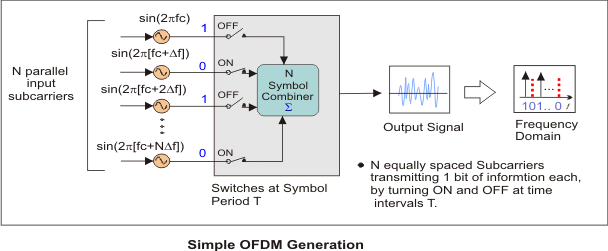
\includegraphics[width=\textwidth]{figures/ofdm-simplegenerator.png}
  \caption{Modulation of signals using OFDM technique \textbf{[source: Keysight]}}
  \label{fig:OFDMGenerator}
\end{figure}
%% TODO : Remove image integrated caption !!
\indent The most basic of these principles is the FDM (\textit{Frequency Division Multiplexing}). It consists in modulating several ($N$) signals using a QAM (\textit{Quadrature Amplitude Modulation}) scheme, with sub-carriers that are regularly spaced by $\Delta f$, see \figref{fig:OFDMGenerator}.
All these modulated signals are then put into an IFFT (\textit{Inverse Fast Fourier Transform}) and summed into a single signal, updated periodicly according to the symbol period $T$ and sent through the desired medium. At the receiver end, the inverse procedure is applied.\\
%
\indent The second main concept is the orthogonality of the sub-carriers. When passing to the frequency domain, each sub-carrier will result in a sinc function. Therefore, the spacing, $\Delta f$, between each of them is chosen so that, in frequency domain, each sub-carrier overlap the others orthogonally, which means all the sinc functions have zero crossing and their side-loops cancel each other, while peaks remain distinguishable, see \figref{fig:freqOrthoSinc}.
%
\begin{figure}[H]
  \centering
  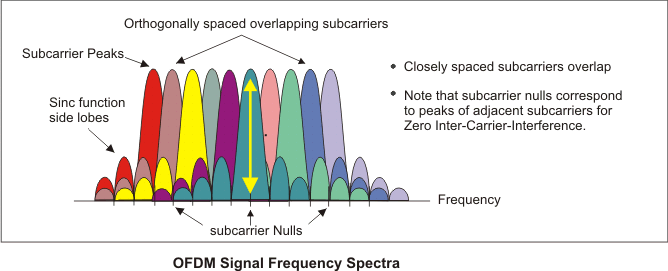
\includegraphics[width=\textwidth]{figures/ofdm-orthogonalspacedsubcarriers.png}
  \caption{Frequency spectrum of OFDM signal \textbf{[source: Keysight]}}
  \label{fig:freqOrthoSinc}
\end{figure}
%
Since, there is no undesirable interference due to frequency overlapping, the spacing between each sub-carrier can be very short. To maintain the orthogonality, this spacing, $\Delta f$, actually has to be the inverse of a symbol period, $T$ :
\begin{flalign}
\eq{\Delta f}{1/T}
\end{flalign}\\
\indent Coming from this relation, and by sending information on parallel channels, it is possible to increase the overall data rate and therefore, the spectral efficiency, while decreasing the data rate on each subchannel. This helps to reduce potential inter-symbol interferences (ISI) at the receiver end, that could happen due to wave reflection, refraction or other multi-path phenomena \cite{RadioElOFDM} and is reinforced by a guard interval between each symbol.\\
%
\indent However, one of the worst disadvantages of OFDM is the high peak-to-power ratio which makes the use of this technique inefficient in terms of energy for small and portable devices.     % OFDM description
% OFDMA description and comparison with OFDM  
\section{What does OFDMA bring ?}
%
\indent OFDMA stands for \textit{Orthogonal Frequency Division Multiple Access}. It allows multiple users to communicate at the same time while keeping the high data rates offered by OFDM.\\
%
\indent The base principle of OFDMA consists in sharing the time and frequency resources between users. It can somehow be compared to a combination of OFDM, FDMA (\textit{Frequency Division Multiple Access}) and TDMA (\textit{Time Division Multiple Access})\cite{WikiOFDMA}. Users are assigned a subset of sub-carriers in the given frequency range and use it for a certain time before it is attributed to another user.\\
\indent All communications can happen in parallel and the attribution of sub-channels is made independently one from another : they can take place at different times and involve different size of sub-channels, see \figref{fig:OFDMvsOFDMA}.\\
%
\begin{figure}[H]
  \centering
  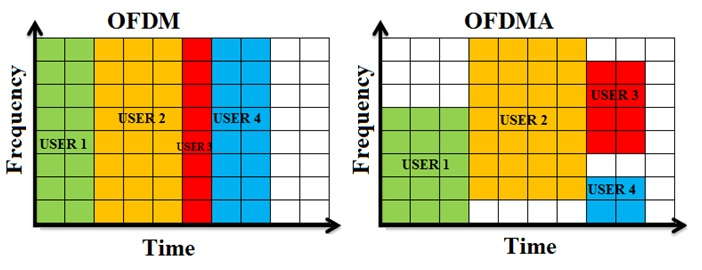
\includegraphics[width=\textwidth]{figures/difference-between-ofdm-and-ofdma.jpg}
  \caption{Comparison between OFDM and OFDMA \textbf{[source: differencebetween.com]}}
  \label{fig:OFDMvsOFDMA}
\end{figure}
%
\indent OFDMA still keeps a strong disadvantage from OFDM which is the high peak-to-average power ratio which makes the use of this technique inefficient in terms of energy for small and portable devices. Despite this fact, OFDMA communication technique has been chosen for 4G LTE networks, designed especially for mobile communications (voice calls, video calls and streaming, World Wide Web access, ...). The next chapter explains briefly how this is achieved.

\paragraph*{See also,}
\cite[Chap.~19]{AMolisch}.
 % OFDMA description and comparison with OFDM  

% Chapter 2 : OFDMA in 4G-LTE Mobile Networks
% Link between OFDMA technique and 4G-LTE
\chapter{OFDM in 4G-LTE Mobile Networks}

\indent 4G-LTE (\textit{4th Generation-Long Term Evolution}, or \textit{3GPP-LTE}, here designated as LTE) is the commercial name of a standard for a communication protocol (physical layer), developed by the 3GPP (\textit{3rd Generation Partnership Project}) and released progressively in different countries around the world, since first launch in Stockholm and Oslo in 2009.

\section{4G-LTE Overview}
%
\indent LTE has been designed as an evolution to former mobile communication techniques (GSM, UMTS, CDMA2000) `to increase 
data rates, improve spectrum efficiency, improve coverage, and reduce latency'\cite{EDahlman}. 4G-LTE was not actually intended to be a proper 4th Generation technology by the 3GPP consortium. However, the initial goal of this \textit{Long Term Evolution} technology is to ensure that 3G can stay competitive throughout years.\\
\indent For instance, one of its definition items actually states that it should reach a \si{100\ Mbps} for the downlink and \si{50\ Mbps} for the uplink and can therefore be used both for voice and data. The difference between the uplink and downlink can be explained with the fact that two slightly different technologies are used.

\section{LTE Technical Considerations}
%
\indent Since, mobile communications usually operate between a BS and a MS (\textit{Mobile Station}), the LTE standard defines rules that accounts for the constraints and advantages of both sides. While, BS don't face the issues from high power-consumption, MS for instance, need a communication technology that doesn't drain all their available power.\\
%
\indent Thus, OFDMA communication technique, described in \secref{sec:OFDMA}, is used as is on the BS side, which allows for \textit{Muliple Access}, to respond a network cell's needs in high traffic and convenient data rates.\\
%
\indent These throughputs can be achieved by chosing the right symbol rate, which is directly influenced by the frequency separation between each subcarrier and therefore, by the number of subcarriers in a channel. Different channel bandwidths are defined in LTE\cite{RadioElLTE}:
\begin{itemize}
  \setlength\itemsep{0.2em}
  \item  1.4 MHz
  \item  3 MHz
  \item  5 MHz
  \item  10 MHz
  \item  15 MHz
  \item  20 MHz.
\end{itemize}
\indent Meanwhile, the sub-carrier spacing, $\Delta f$, is set to \si{15\ kHz}, which yields \si{15\ ksps} and a symbol time of:
\begin{flalign}
\eq{T_S}{\frac{1}{15 \cdot 10^3}}&\nonumber\\
\eq{T_S}{66,7 \cdot 10^{-6}}\si{s}&\nonumber \\
\eq{T_S}{66,7}\si{\mu s}.&\nonumber
\end{flalign}\\ 
\indent Eventually, using a \si{20\ MHz} channel bandwidth (which allows for 100 frequency resource blocks of 12 subcarriers) and a 64QAM (which means 6 bits are used to map bits of data in one symbol), results in having a theoretical data rate of \si{108\ Mbps}. However, the signal being affected by several physical and environmental factors, the real data rate is actually lower.\\
\indent Moreover, the cycling prefix, $T_{CP}$, used by OFDM to reduce ISI even more than allowed by the low symbol time, is defined for LTE as :
\begin{flalign}
\eq{T_{CP}}{4,69}\si{\mu s}.&\nonumber
\end{flalign}\\ 
%
\indent While simple OFDMA happens at BS side, and the previously defined standards remain the same, the technique used on the MS side is slightly modified into what is called SC-FDMA (\textit{Single Carrier - Frequency Division Multiple Access}), which allows to lower the peak-to-average ratio and thus, reduce the power consumption over time. This is achieved by having the users (MS) to apply a supplementary DFT before bit mapping (compensated on the receiver end by an IDFT after de-mapping) and use a single-carrier structure, see \figref{fig:SCFDMAGenerator}.
%
\begin{figure}[H]
  \centering
  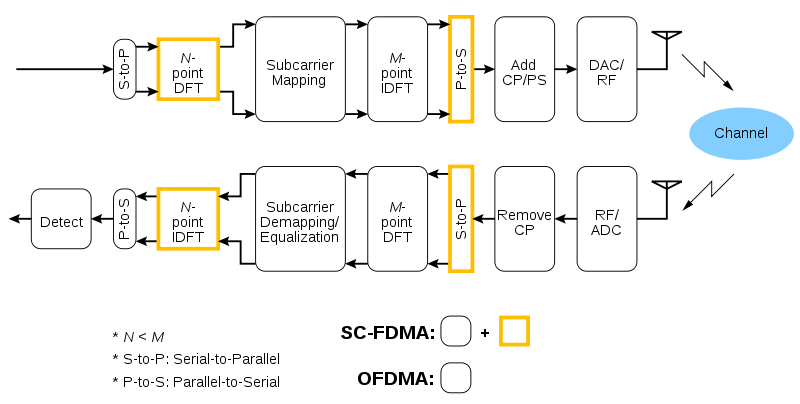
\includegraphics[width=\textwidth]{figures/SC-FDMA.png}
  \caption{SC-FDMA signal generation\textbf{[source: Wikipedia]}}
  \label{fig:SCFDMAGenerator}
\end{figure}

%%% Setup for Appendix and Bibliography %%%
\addtocontents{toc}{\bigskip}

%%% Bibliography %%%
\printbibliography

\end{document}